\section{PCF and Gap-Junction Response to Constant Stimulus}

We compute the response of the PCF and GJ models to a constant driving stimulus as we did for the SC model in section (\ref{section:analysis:sc_rmse})
 
\subsection{PCF Network Response to Constant Stimulus:}
To compare between PCF and SC, we consider the same dynamical system as before, but using unrotated bases i.e.

$$
\dot{x} = Ax + Bc, \hspace{4mm} x(0) = x_0
$$

where,

$$
A = \mathcal{U} \Lambda \mathcal{U}^T,
$$

and the neuron encoding directions are 
$$
D = \mathcal{U} \begin{bmatrix} S & 0 \end{bmatrix} V^T = \begin{bmatrix} d_1 & \hdots & d_N \end{bmatrix} \in \mathbf{R}^{d \times N}.
$$


We choose $c$ such that 

$$
x = k \frac{d_j}{||d_j||}
$$

is a fixed point, i.e. 

%ax + bc = 0 --> -bc = ax  --> - 1/a b c = x --> c =  - 1/b a x 

\begin{align*}
\dot{x} &= 0
\\
\\
\implies
c &= -\frac{k}{||d_j||} B^{-1}A d_j,  \hspace{4mm} k \in \mathbf{R}.
\end{align*}

The network error is $e = x - \hat{x}$ consequently grows parallel to $d_j$, ensuring only neuron $j$ spikes periodically.

The spike train $o_j$ becomes a periodic sequence of impulses spaced in time by $\frac{1}{\phi_j}$. If the first spike occurs at $\xi_j^0 = 0$, then $\o_j(\xi) = \sum_{l=0}^{\infty} \delta \left(\xi-\frac{l}{\phi_j}\right).$ Since only neuron $j$ spikes, the estimate is

\begin{align*}
\dot{\hat{x}}(\xi) = - \hat{x} + \sum_{l=0}^{\infty} \delta \left(\xi_j^k - \frac{l}{\phi_j}\right) \, d_j .
\end{align*}

Using an identical inductive approach as before, the PCF network steady state estimate is 

\begin{equation}
\label{eq:analysis:pcf_gj_const_driving:estimate_explicit_phi}
\hat{x}(\xi) =
\frac{d_j}{1 - e^{-\frac{1}{\phi_j}}} e^{- (\xi) \mod{\frac{1}{\phi_j}}},
\end{equation} 
where $x \mod{y}$ denotes the fractional remainder of $x$ after division by $y$. 
\\
\\
We compute the  RMSE of the error $e$ by 
\begin{align*}
RMSE = \sqrt{\phi_j \int_{0}^{\frac{1}{\phi_j}} \!  ||e(\tau)||^2 \, \, \mathrm{d}\tau}.
\end{align*}

The integrand simplifies to 

\begin{align*}
||e||^2  &= (x - \hat{x})^2 
\\
\\
&= ||x||^2 - 2 x^T\hat{x} + ||\hat{x}||^2
\\
\\
&= 
k^2 - 2\frac{k}{1 - e^{-\frac{1}{\phi_j}}} ||d_j|| e^{-\tau} + \left(\frac{||d_j||}{1 - e^{-\frac{1}{\phi_j}}}\right)^2 e^{-2\tau}
\\
\\
\end{align*}

This gives an RMSE of 

$$
RMSE(k, d_j, \phi_j) = 
\sqrt{
k^2 - 2 \phi_j \, k ||d_j|| +\phi_j \, ||d_j||^2 \frac{1 + e^{-\frac{1}{\phi_j}}}{1 - e^{-\frac{1}{\phi_j}}}.
}
$$

To simplify, note that immediately before a spike, 

\begin{align*}
d_j^T e &= d_j^T \left(k \frac{d_j}{||d_j||}  - d_j \frac{e^{-\frac{1}{\phi_j}}}{1 - e^{-\frac{1}{\phi_j}}}\right) 
\\
\\
&= \frac{||d_j||^2}{2}
\\
\\
\implies
 \frac{||d_j||^2}{2} &= d_j^T \left(k \frac{d_j}{||d_j||}  - d_j \frac{e^{-\frac{1}{\phi_j}}}{1 - e^{-\frac{1}{\phi_j}}}\right)
\\
\\
\implies 
e^{\frac{1}{\phi_j}} - 1 &= \frac{1}{\frac{k}{||d_j||} - \frac{1}{2}} 
\\
\\
\implies
\frac{{1 + e^{-\frac{1}{\phi_j}}}}{{1 - e^{-\frac{1}{\phi_j}}}} 
&=
\frac{2 \, k}{||d_j||}.
\end{align*}

Combine this with the RMSE expression to get 

\begin{align*}
RMSE(\phi_j, k) = 
k \sqrt{
	1 - 2 \phi_j tanh \left(\frac{1}{2 \, \phi_j} \right)
}. 
\end{align*}

Divide by driving strength $k$ to get the dimensionless quantity that depends only on spike rate, 

\begin{align}
\label{eq:analysis:pcf_gj_const_driving:nrmse}
NRMSE(\phi_j) = 
\sqrt{
	1 - 2 \phi_j tanh \left(\frac{1}{2 \, \phi_j} \right)
}. 
\end{align}

Equation (\ref{eq:analysis:pcf_gj_const_driving:nrmse}) is identical to the self-coupled network RMSE, equation (\ref{eq:const_driving:per_spike_rmse_phi}) and is plotted against numerical simulations of a PCF network in figure (\ref{fig:const_driving:pcf_nrmse_vs_phi})

\begin{figure}
\centering
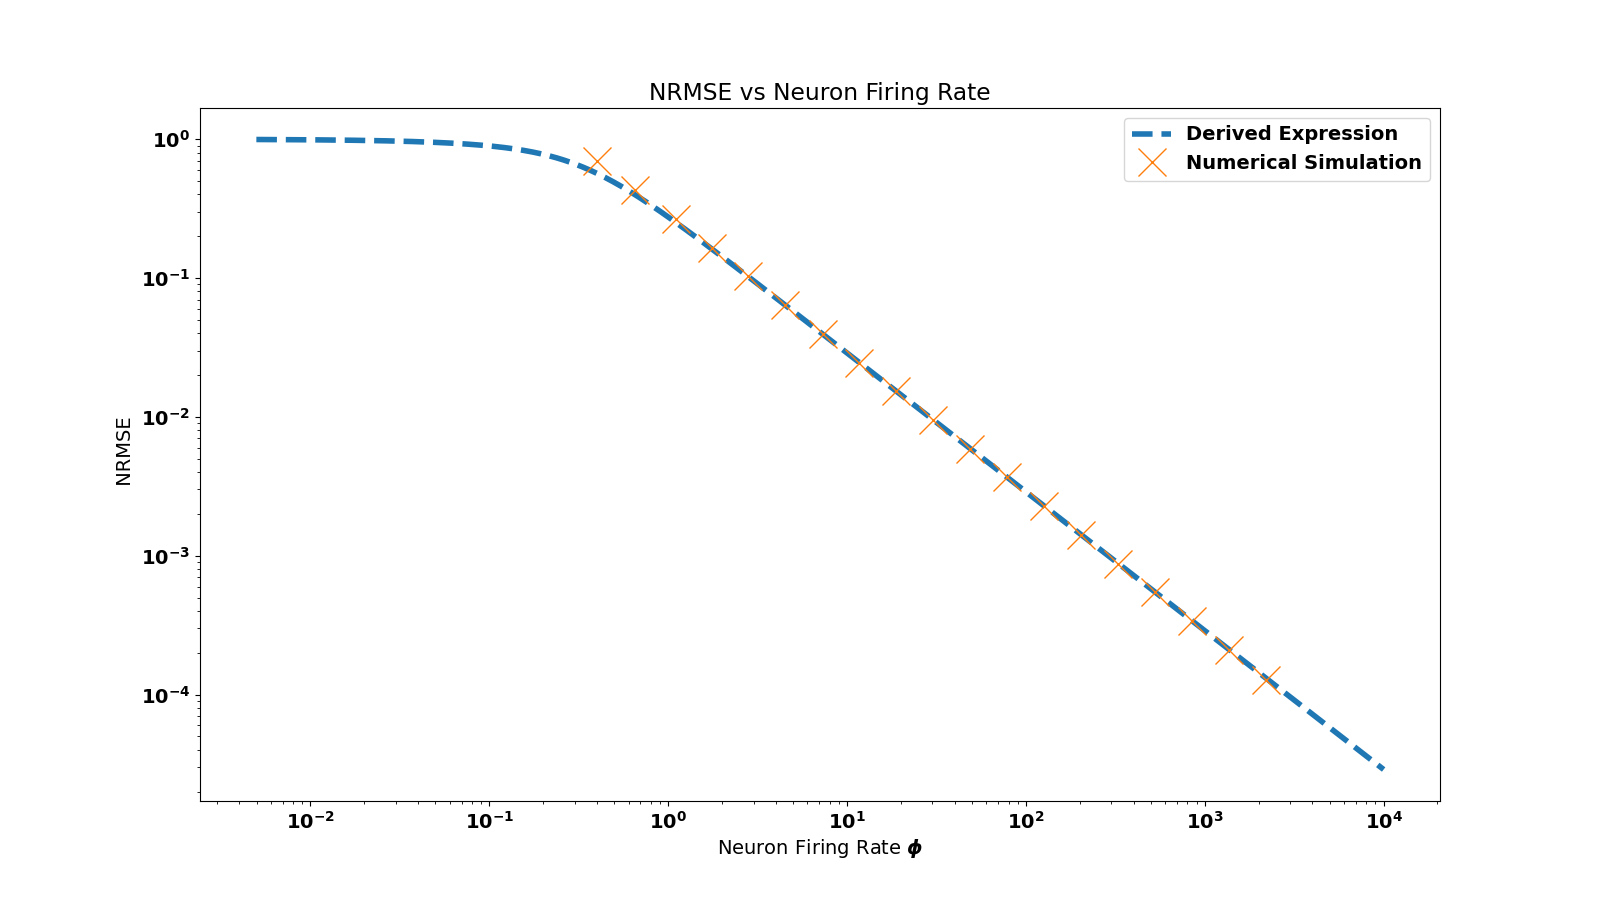
\includegraphics[width=\linewidth]{figures/pcf_nrmse_vs_phi}
\caption{Log-log Plot of Equation (\ref{eq:analysis:pcf_gj_const_driving:nrmse}). The RMSE was computed numerically by the discrete integral $RMSE = \sqrt{\frac{1}{\phi} \sum_{i} (x - \hat{x})^2 d\xi}$, where $i$ sums over the data points in a spike. The integration is performed over $n = 100$ interspike intervals and averaged to form a data point. The time step was $d\xi = 10^{-4}$.}
\label{fig:const_driving:pcf_nrmse_vs_phi}
\end{figure}


\subsection{Gap-Junction Network Response to Constant Stimulus:} 

We now implement the same dynamical system as before with a GJ network. 
As with the PCF network, we drive the GJ network such that the fixed point is $x = k\frac{d_j}{||d_j||}$ parallel to neuron $j$, 

$$
\dot{x} = 0 \implies c = -\frac{k}{||d_j||}B^{-1}A d_j. 
$$
This reduces the network to only neuron $j$ spiking periodically. 

The spike train $o_j$ becomes a periodic sequence of impulses spaced in time by $\frac{1}{\phi_j}$. If the first spike occurs at $\xi_j^0 = 0$, then $\o_j(\xi) = \sum_{l=0}^{\infty} \delta \left(\xi-\frac{l}{\phi_j}\right).$ Since only neuron $j$ spikes, the estimate is

\begin{align*}
\dot{\hat{x}}(\xi) = - \hat{x} + \sum_{l=0}^{\infty} \delta \left(\xi_j^k - \frac{l}{\phi_j}\right) \, d_j .
\end{align*}

Note that this estimate is identical to the PCF estimate above. Following the same procedure, we arrive at the GJ NRMSE:

\begin{align}
\label{eq:analysis:pcf_gj_const_driving:nrmse}
NRMSE(\phi_j) = 
\sqrt{
	1 - 2 \phi_j tanh \left(\frac{1}{2 \, \phi_j} \right)
}. 
\end{align}

Equation (\ref{eq:analysis:pcf_gj_const_driving:nrmse}) is identical to the self-coupled network RMSE, equation (\ref{eq:const_driving:per_spike_rmse_phi}) and is plotted against numerical simulations of a PCF network in figure (\ref{fig:const_driving:gj_nrmse_vs_phi})

\begin{figure}
\centering
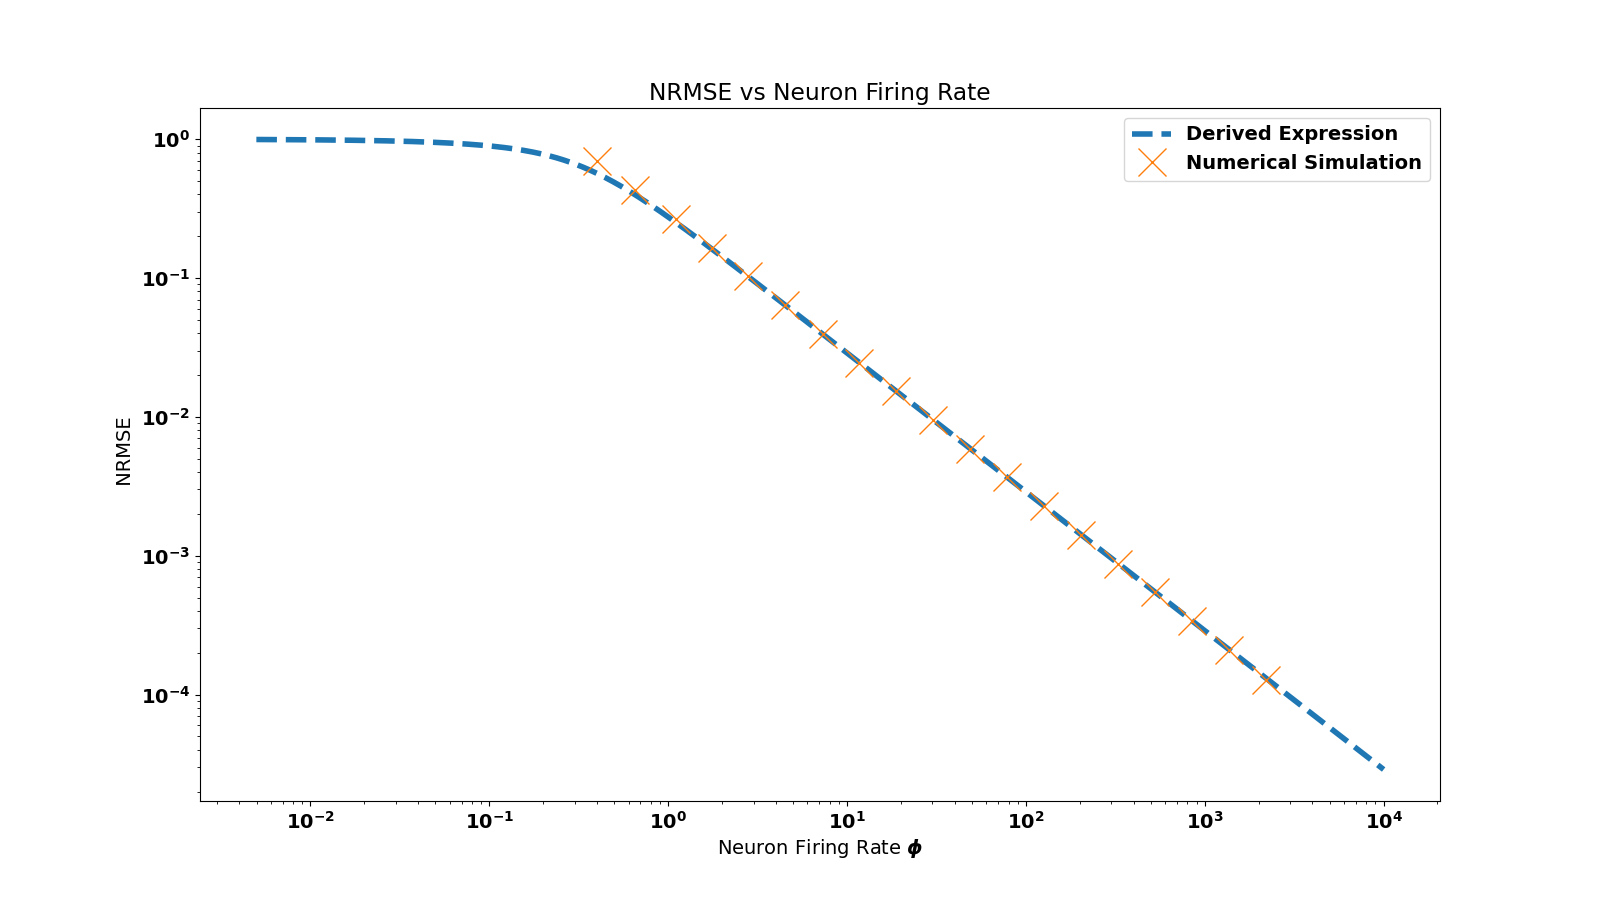
\includegraphics[width=\linewidth]{figures/pcf_nrmse_vs_phi}
\caption{Log-log Plot of Equation (\ref{eq:analysis:pcf_gj_const_driving:nrmse}). The RMSE was computed numerically by the discrete integral $RMSE = \sqrt{\frac{1}{\phi} \sum_{i} (x - \hat{x})^2 d\xi}$, where $i$ sums over the data points in a spike. The integration is performed over $n = 100$ interspike intervals and averaged to form a data point. The time step was $d\xi = 10^{-4}$.}
\label{fig:const_driving:gj_nrmse_vs_phi}
\end{figure}


\clearpage

\subsection{Comparison of Self-Coupled, Gap-Junction, and PCF Networks for a Constant Stimulus}

We now compare all three models as they respond to a constant driving stimulus. Each is driven parallel to a single neuron $j$. As we showed, each results in an NRMSE given by 

$$
NRMSE(\phi_j) = 
\sqrt{
	1 - 2 \phi_j tanh \left(\frac{1}{2 \, \phi_j} \right)
}. 
$$
 
 
To validate numerically, we simulate the SC, PCF, and GJ networks using the same network parameters. Next we compare each NRMSE as predicted by the equation above with numerical measurements. This is shown in figure (\ref{fig:analysis:comparison_sc_vs_pcf_vs_gj:per_spike_rmse_sc_pcf_gj}). Note that while the relationship between firing rate and NRMSE is the same, the firing rate under a given set of parameters is not the same between networks. 


\clearpage 


\begin{figure}
\centering
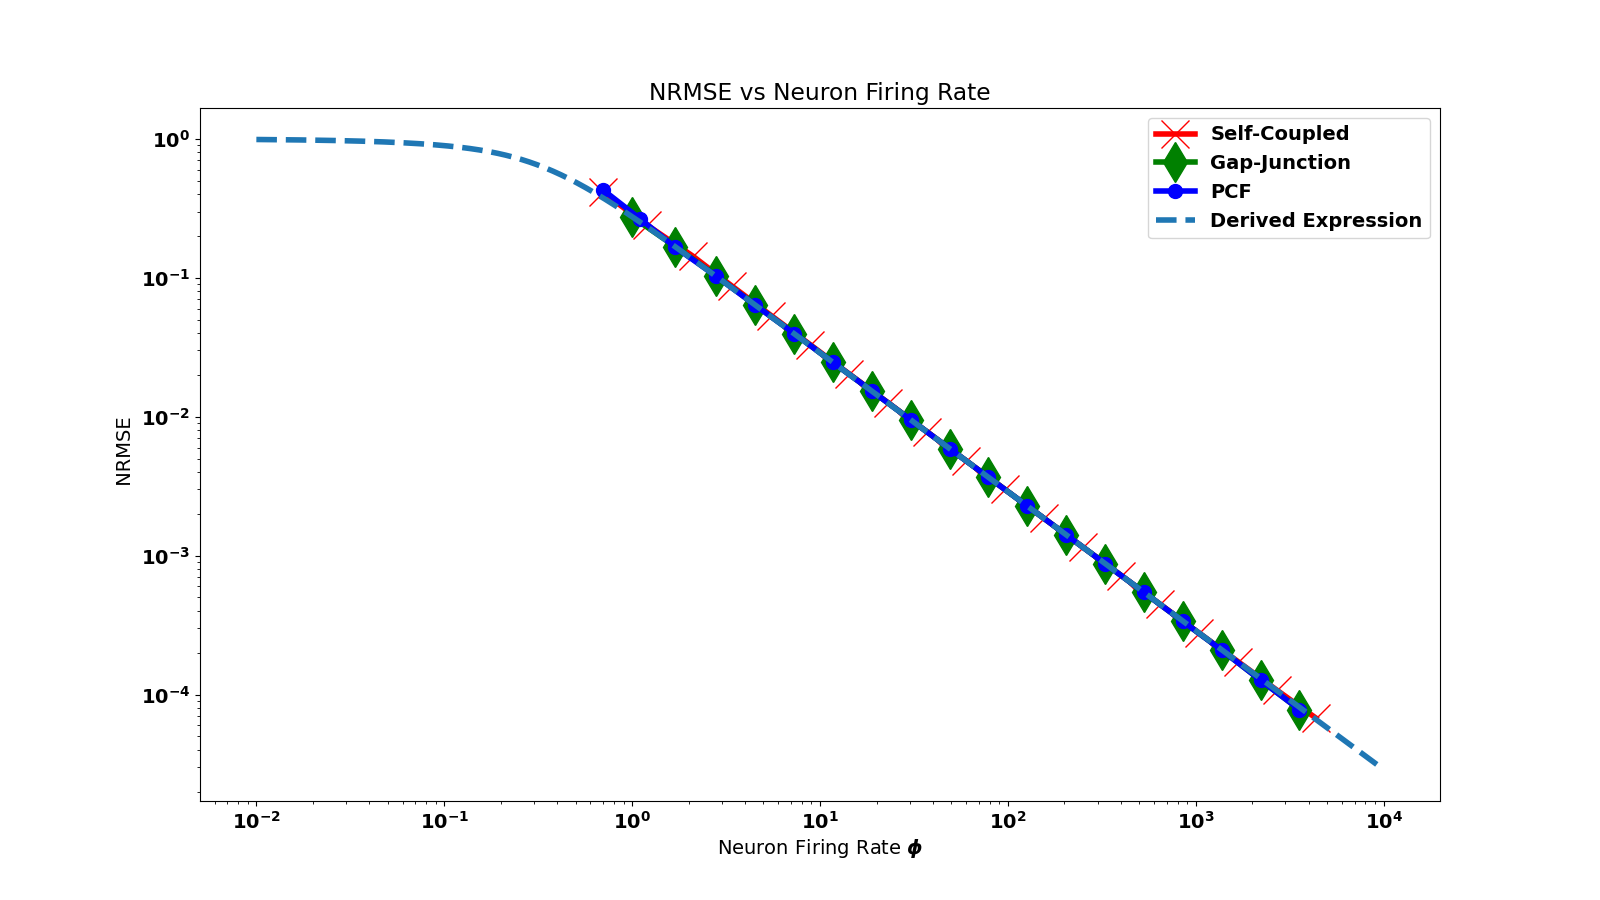
\includegraphics[width=\linewidth]{figures/sc_pcf_gj_nrmse_vs_phi}
\caption{Simulated RMSE for self-coupled, gap-junction, and PCF networks. The dotted line is the derived expression for each model given by given above. Spike rates were estimated numerically by dividing the number of spikes by the simulation length. The RMSE was computed numerically by the discrete integral $\hat{RMSE} = \sqrt{\hat{\phi} \sum_{\tau \text{ between spikes }} e(\xi)^T e(\xi) \, \, d\xi }$. All computations used the numerically estimated spike rate.} 
\label{fig:analysis:comparison_sc_vs_pcf_vs_gj:per_spike_rmse_sc_pcf_gj}
\end{figure}

